

\newcommand{\molecule}[3]{%
\draw (\x1,0) circle (0.3) node {#1};
\draw (\x2,0) circle (0.3) node {#2};
\draw (\xm,0) ellipse (\e1 and \e2);

\begin{scope}
    \clip (\xm,0) rectangle ++#3;
    \draw[line width = 2pt] (\xm,0) ellipse (\e1 and \e2);
\end{scope}
}

  
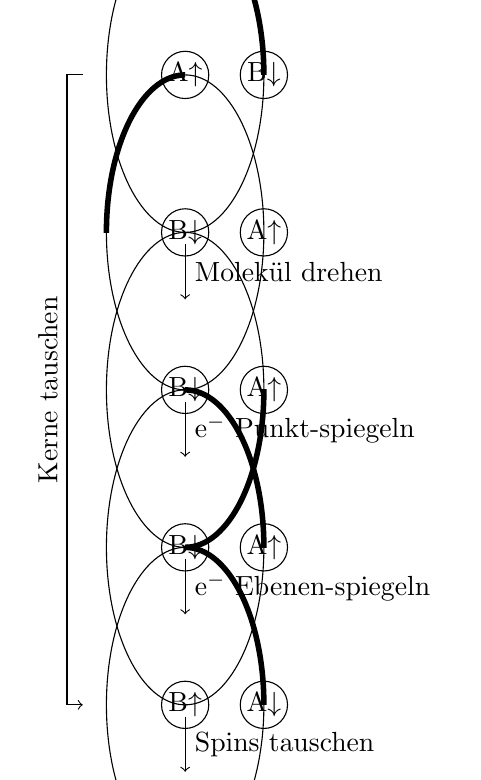
\begin{tikzpicture}
\useasboundingbox (-1.,-0.6) rectangle (4.4,8.6);
%	\draw (-1.,-0.8) rectangle (4.4,8.8);
  \tikzmath{\x1 = 0.7; \x2 = 1.7; \e1=1.3; \e2=0.5;}
  \tikzmath{\xm = (\x1 + \x2) / 2; }
  

\begin{scope}[yshift=8cm,local bounding box=b1]
    \molecule{A$\uparrow$}{B$\downarrow$}{(3,3)}
    \draw[->](\xm,-\e2 - 0.15) -- node[anchor=west] {Molekül  drehen} ++(0,-0.7) ;
\end{scope}


\begin{scope}[yshift=6cm, local bounding box=b2]
    \molecule{B$\downarrow$}{A$\uparrow$}{(-3,3)}
    \draw[->](\xm,-\e2 - 0.15) -- node[anchor=west] {e$^-$ Punkt-spiegeln} ++(0,-0.7) ;
\end{scope}

\begin{scope}[yshift=4cm]
    \molecule{B$\downarrow$}{A$\uparrow$}{(3,-3)}
      \draw[->](\xm,-\e2 - 0.15) -- node[anchor=west] {e$^-$  Ebenen-spiegeln} ++(0,-0.7) ;
\end{scope}

\begin{scope}[yshift=2cm]
    \molecule{B$\downarrow$}{A$\uparrow$}{(3,3)}
      \draw[->](\xm,-\e2 - 0.15) -- node[anchor=west] {Spins tauschen} ++(0,-0.7) ;
\end{scope}


\begin{scope}
    \molecule{B$\uparrow$}{A$\downarrow$}{(3,3)}
\end{scope}
 
\draw[->] (-0.3,8) -- ++ (-0.2,0) -- node[rotate=90, anchor=south] {Kerne tauschen} ++(0,-8) -- ++ (0.2,0);
 
\end{tikzpicture}

